\documentclass[tikz, border=5pt]{standalone}
\usetikzlibrary{positioning}

\begin{document}

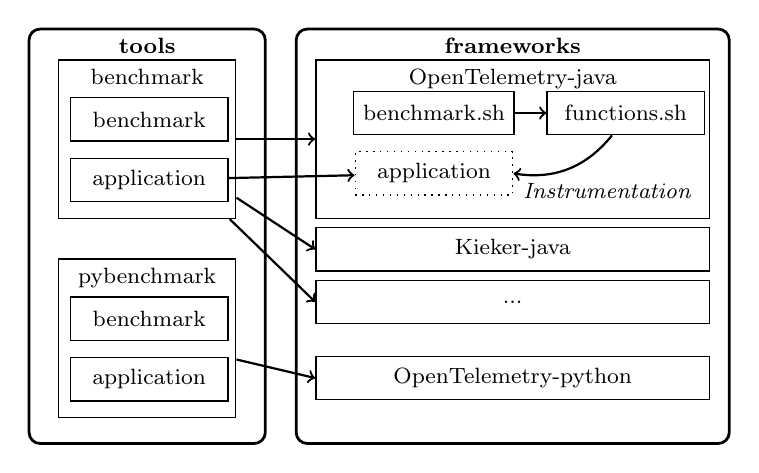
\begin{tikzpicture}[node distance = 0.4cm, auto, font=\footnotesize, align=center, 
  every node/.style={line width=0.5pt,draw,shape=rectangle,minimum width = 2.85cm, minimum height=0.55cm, align=center},
  framework/.style={draw, minimum width=5.0cm, shape=rectangle},
  component/.style={draw, minimum width=2.0cm, shape=rectangle}]

      \node[shape=rectangle, minimum width=2.25cm] (benchmarkJ) {benchmark\\[1.25cm]};
      
      \node[component, right=0.15cm of benchmarkJ.west, yshift=0.25cm] (benchmark) {benchmark};
      \node[component, below=0.2cm of benchmark] (application) {application};

      \node[shape=rectangle, minimum width=2.25cm, below=0.5cm of benchmarkJ] (pybenchmark) {pybenchmark\\[1.25cm]};
      \node[component, right=0.15cm of pybenchmark.west, yshift=0.25cm] (benchmark2) {benchmark};
      \node[component, below=0.2cm of benchmark2] (application2) {application};

      \node (OpenTelemetry-java) [framework, right=1.0cm of benchmarkJ.north east, anchor=north west] {OpenTelemetry-java\\[1.25cm]};
      \node (Kieker-java) [framework, below=0.1cm of OpenTelemetry-java] {Kieker-java};
      \node (other) [framework, below=0.1cm of Kieker-java] {...};
      \node (OpenTelemetry-python) [framework, below=of other] {OpenTelemetry-python};

      \node[above=of benchmarkJ.north, anchor=north, align=center, rounded corners, minimum width=3.0cm, line width=1pt] (tools) {\textbf{tools}\\[4.5cm]};
      \node[above=of OpenTelemetry-java).north east, xshift=0.0cm, anchor=north, align=center, rounded corners, minimum width=5.5cm, line width=1pt] (tools) {\textbf{frameworks}\\[4.5cm]};
      %\draw[draw, rounded corners, line width=1pt] ($(Kieker-java-aspectj.north west) - (0.15, -0.5cm)$) rectangle ($(Kieker-java-aspectj.north east) - (-2.75, 1.5cm)$) node [draw=none,pos=.2,xshift=-1.25cm] {\textbf{frameworks}};

      \draw [->, thick] (benchmarkJ) -- (Kieker-java.west);
      \draw [->, thick] (benchmarkJ) -- (OpenTelemetry-java.west);
      \draw [->, thick] (benchmarkJ) -- (other.west);
      \draw [->, thick] (pybenchmark) -- (OpenTelemetry-python.west);
      
      \node[component, below=of OpenTelemetry-java.north, xshift=-1cm] (benchmarkSH) {benchmark.sh};
      \node[component, right=of benchmarkSH] (functionsSH) {functions.sh};
      \node[component, dotted, below=0.2cm of benchmarkSH]  (applicationInstrumented) {application};
      
      \draw [->, thick] (benchmarkSH) -- (functionsSH);
      \draw [->, thick] (application) -- (applicationInstrumented);
      
      \draw (functionsSH) edge [bend left, ->, thick] node [below, draw=none, xshift=0.5cm] {\textit{Instrumentation}} (applicationInstrumented.east);
\end{tikzpicture}

\end{document}
